\chapter{Optimization of $b$-tagging working point in $\FourBfull$ search}
\label{AppendixA}

To the $3b$ and $4b$ signal regions in the boosted $\FourBfull$ search, the MV2 algorithm with a $20\%$ fraction of charm events in training is used (MV2c20). Once the algorithm is selected, an efficiency working point must also be chosen. This working point defines the efficiency with which true $b$-jets are tagged and also fixes the overall background rejection of the algorithm. Higher efficiency working points accept more true $b$-jets but also allow for more background. Five different working points ($70\%$, $77\%$, $80\%$, $85\%$, $90\%$) are tested. With each working point, the full data driven background estimation method is run to quantify the amount of background that will be present in the final signal region. The significance is quantified using the median discovery significance for signal and background with Poisson errors, given in equation~\ref{eqn:Cowan_sig}~\cite{CowanSig}. 
%
\begin{equation}
\label{eqn:Cowan_sig}
Z = \sqrt{2\left((s+b)\ln\left(1+\frac{s}{b}\right) - s\right)}
\end{equation}
%
Note that in the limit where $s$ is much smaller than $b$, this equation reduces to the more well known $s/\sqrt{b}$. 

Figure~\ref{fig:4b_sig_opt} shows the estimated significance as a function of signal mass in RSG $c=1$ models for the $3b$ and $4b$ signal regions. The $77\%$ working point gives the best performance over a wide range of masses in the $4b$ signal region. As this is the region which contributes the most to the total discovery significance, the $77\%$ efficiency working point is chosen for the analysis. 


\begin{figure}[h!]
  %\vspace{20pt}
  \centering
  \captionsetup{justification=centering}

   \begin{subfigure}[t]{0.5\textwidth}
        \centering
        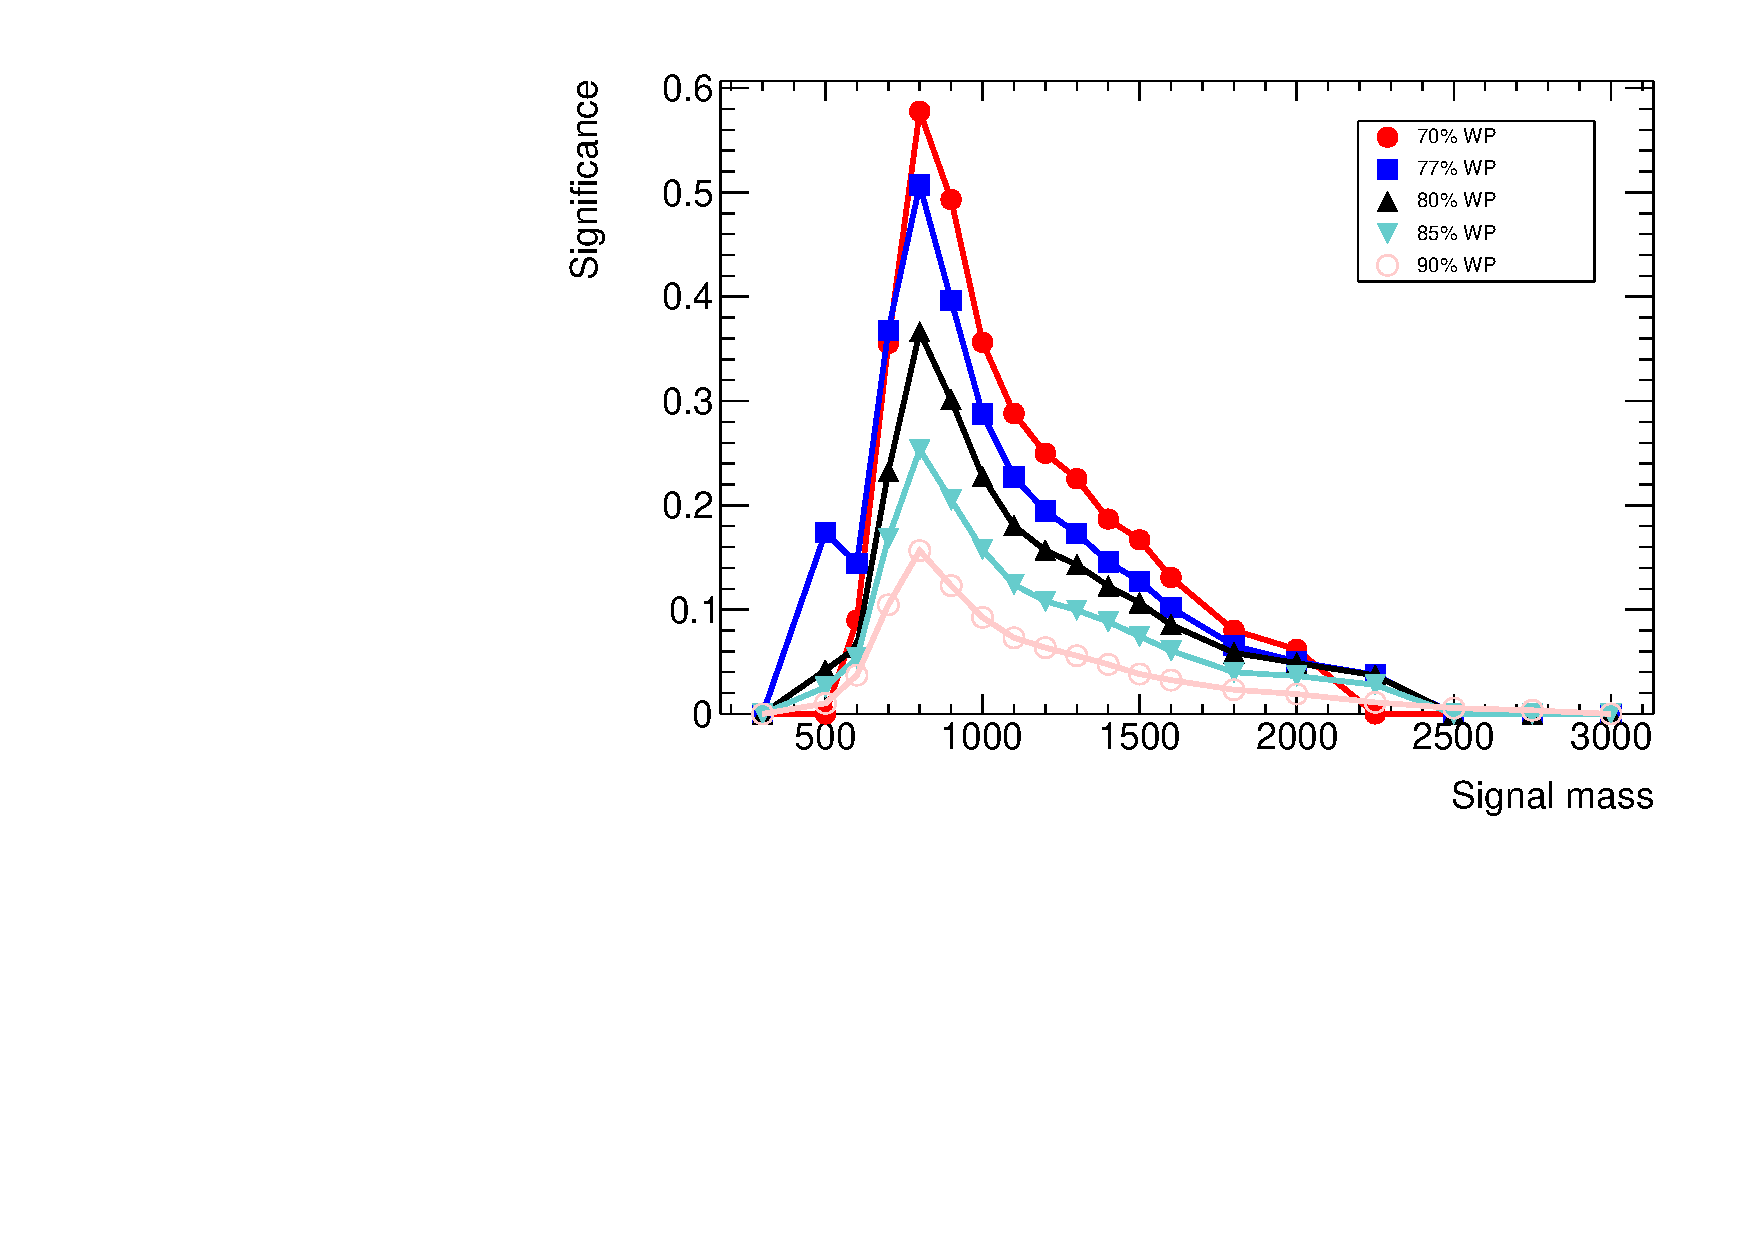
\includegraphics[width=0.7\textwidth,angle=270]{figures/sig_optimization_3b}
        \caption{}
    \end{subfigure}%
    \begin{subfigure}[t]{0.5\textwidth}
        \centering
        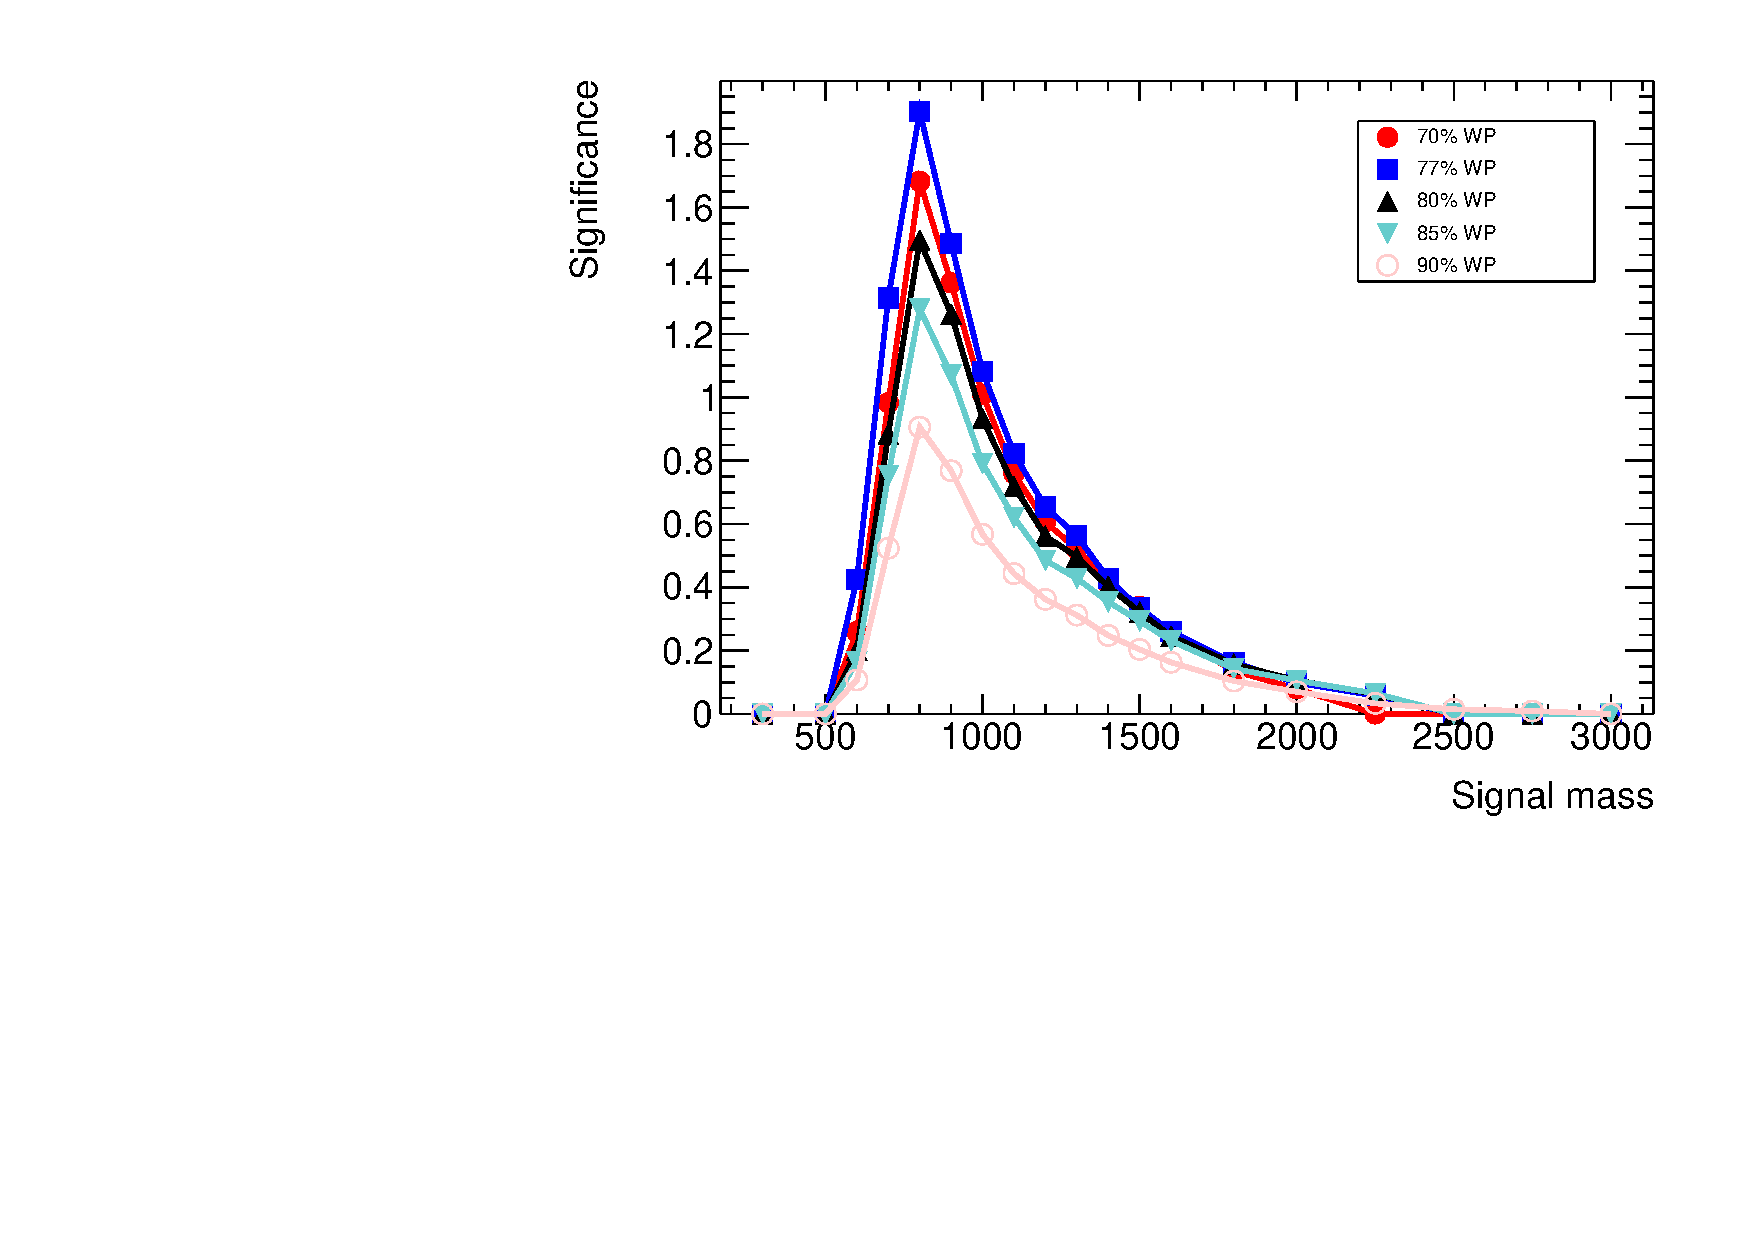
\includegraphics[width=0.7\textwidth,angle=270]{figures/sig_optimization_4b}
        \caption{}
    \end{subfigure}

   \caption{Estimated significance as a function of signal mass for RSG $c=1$ models in the $3b$ (a) and $4b$ (b) regions for different $b$-tagging efficiency working points}
  \label{fig:4b_sig_opt}
\end{figure}
